\documentclass{article}
\usepackage{tikz}
\usepackage{amssymb}
\usetikzlibrary{calc,positioning,arrows.meta,decorations.markings}

% Define custom gamaka markers
\tikzset{
    % Start markers
    gamaka start circle/.style={circle, fill=white, draw=black, inner sep=2pt},
    gamaka start square/.style={rectangle, fill=white, draw=black, inner sep=2pt},
    gamaka start diamond/.style={diamond, fill=white, draw=black, inner sep=2pt},
    gamaka start triangle/.style={regular polygon, regular polygon sides=3, fill=white, draw=black, inner sep=2pt},
    % End markers (filled versions)
    gamaka end circle/.style={circle, fill=black, inner sep=2pt},
    gamaka end square/.style={rectangle, fill=black, inner sep=2pt},
    gamaka end diamond/.style={diamond, fill=black, inner sep=2pt},
    gamaka end arrow/.style={-stealth, thick},
    % Curve styles for different gamakas
    kampita curve/.style={thick, blue, 
        decoration={markings,
            mark=at position 0 with {\node[gamaka start circle] {};},
            mark=at position 1 with {\node[gamaka end circle] {};}
        },
        postaction={decorate}
    },
    jaru curve/.style={thick, red,
        decoration={markings,
            mark=at position 0 with {\node[gamaka start square] {};},
            mark=at position 1 with {\arrow{stealth};}
        },
        postaction={decorate}
    },
    andolita curve/.style={thick, green!60!black,
        decoration={markings,
            mark=at position 0 with {\node[gamaka start diamond] {};},
            mark=at position 1 with {\node[gamaka end diamond] {};}
        },
        postaction={decorate}
    },
    tribhinna curve/.style={thick, purple,
        decoration={markings,
            mark=at position 0 with {\node[gamaka start triangle] {};},
            mark=at position 0.33 with {\fill circle (2pt);},
            mark=at position 0.66 with {\fill circle (2pt);},
            mark=at position 1 with {\arrow{stealth};}
        },
        postaction={decorate}
    }
}

\begin{document}

\section*{Gamaka Notation with Start/End Markers}

\subsection*{Legend}
\begin{tikzpicture}
    \node at (0,0) {Gamaka Types:};
    
    % Kampita
    \draw[kampita curve] (2,0) .. controls (2.5,0.3) and (3.5,0.3) .. (4,0);
    \node[right] at (4.2,0) {Kampita (oscillation)};
    
    % Jaru
    \draw[jaru curve] (2,-0.5) .. controls (2.5,-0.2) and (3.5,-0.8) .. (4,-0.5);
    \node[right] at (4.2,-0.5) {Jaru (glide)};
    
    % Andolita
    \draw[andolita curve] (2,-1) .. controls (2.5,-0.7) and (3.5,-1.3) .. (4,-1);
    \node[right] at (4.2,-1) {Andolita (swing)};
    
    % Tribhinna
    \draw[tribhinna curve] (2,-1.5) .. controls (2.5,-1.2) and (3.5,-1.8) .. (4,-1.5);
    \node[right] at (4.2,-1.5) {Tribhinna (three-part)};
\end{tikzpicture}

\vspace{1cm}

\subsection*{Musical Phrase with Gamakas}
\begin{tikzpicture}[scale=2]
    % Staff lines
    \foreach \y in {0,0.5,1,1.5,2} {
        \draw[gray,thin] (0,\y) -- (8,\y);
    }
    
    % Notes
    \coordinate (Sa) at (1,1);
    \coordinate (Ri) at (2,1.5);
    \coordinate (Ga) at (3,0.5);
    \coordinate (Ma) at (4,1);
    \coordinate (Pa) at (5,1.5);
    \coordinate (Dha) at (6,1);
    \coordinate (Ni) at (7,2);
    
    % Draw notes
    \foreach \n in {Sa,Ri,Ga,Ma,Pa,Dha,Ni} {
        \fill (\n) circle (0.08);
    }
    
    % Gamakas with markers
    \draw[kampita curve] (Sa) .. controls (1.3,1.3) and (1.7,1.7) .. (Ri);
    \draw[jaru curve] (Ri) .. controls (2.5,1.2) and (2.8,0.3) .. (Ga);
    \draw[andolita curve] (Ga) .. controls (3.3,0.8) and (3.7,1.2) .. (Ma);
    \draw[tribhinna curve] (Ma) .. controls (4.5,1.3) and (4.8,1.6) .. (Pa);
    
    % Labels
    \node[below=3pt] at (Sa) {Sa};
    \node[above=3pt] at (Ri) {Ri};
    \node[below=3pt] at (Ga) {Ga};
    \node[below=3pt] at (Ma) {Ma};
    \node[above=3pt] at (Pa) {Pa};
    \node[below=3pt] at (Dha) {Dha};
    \node[above=3pt] at (Ni) {Ni};
\end{tikzpicture}

\vspace{1cm}

\subsection*{Complex Gamaka Patterns}
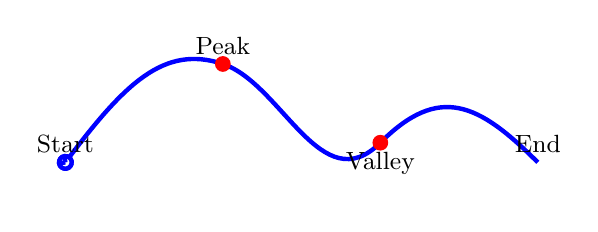
\begin{tikzpicture}[scale=2.5]
    % Custom arrow tips for different gamaka endings
    \tikzset{
        start marker/.style={
            decoration={markings,
                mark=at position 0 with {
                    \draw[fill=white] (0,0) circle (0.08);
                    \draw (0,0) -- (0.05,0.05);
                    \draw (0,0) -- (-0.05,0.05);
                }
            },
            postaction={decorate}
        },
        end marker/.style={
            decoration={markings,
                mark=at position 1 with {
                    \draw[-stealth,thick] (-0.1,0) -- (0,0);
                }
            },
            postaction={decorate}
        }
    }
    
    % Complex curve with multiple control points
    \draw[ultra thick, blue, start marker, end marker] 
        (0,0) .. controls (0.3,0.4) and (0.5,0.6) .. (0.8,0.5)
              .. controls (1.1,0.4) and (1.3,-0.2) .. (1.6,0.1)
              .. controls (1.9,0.4) and (2.1,0.3) .. (2.4,0);
    
    % Add intermediate markers
    \fill[red] (0.8,0.5) circle (0.04);
    \fill[red] (1.6,0.1) circle (0.04);
    
    % Annotations
    \node[above] at (0,0) {\small Start};
    \node[above] at (2.4,0) {\small End};
    \node[above] at (0.8,0.5) {\small Peak};
    \node[below] at (1.6,0.1) {\small Valley};
\end{tikzpicture}

\end{document}